\documentclass[12pt]{report}

\usepackage{amssymb, fullpage, amsmath,mathtools}
\usepackage{graphicx}

\newtheorem{problem}{Problem}

\newenvironment{solution}[1][\it{Solution}]{\textbf{#1. } }{$\square$}

\graphicspath{ {./} }

\allowdisplaybreaks

\pagestyle{empty}

\def\Z{{\mathbb Z}}
\def\Q{{\mathbb Q}}
\def\C{{\mathbb C}}
\def\R{{\mathbb R}}
\def\N{{\mathbb N}}
\def\eps{{\epsilon}}
\def\O{{\mathcal{O}}}
\def\half{\frac{1}{2}}
\newcommand{\floor}[1]{{\left\lfloor#1\right\rfloor}} % Floor function
\newcommand{\ceil}[1]{{\left\lceil#1\right\rceil}} % Ceiling function
\newcommand{\paren}[1]{{\left(#1\right)}} % Parentheses ()
\newcommand{\brac}[1]{{\left\{#1\right\}}} % Curly braces {}
\newcommand{\braces}[1]{{\left[#1\right]}} % Braces []
\newcommand{\abrac}[1]{{\left\langle#1\right\rangle}} % Angle Braces <>
\newcommand{\abs}[1]{{\left|#1\right|}} % Absolute value
\newcommand{\norm}[1]{{\left\|#1\right\|}} % Norm
\newcommand{\eval}[2]{\right|_{#1}^{#2}} % Evaluate

\newcommand{\pp}[2]{\frac{\partial #1}{\partial #2}} % Partial of 1 wrt 2
\newcommand{\ppn}[3]{\frac{\partial^{#1} #2}{\partial #3^{#1}}} % nth Partial of 1 wrt 2
\newcommand{\dd}[2]{\frac{\mathrm{d} #1}{\mathrm{d} #2}} % Partial of 1 wrt 2
\newcommand{\ddn}[3]{\frac{\mathrm{d}^{#1} #2}{\mathrm{d} #3^{#1}}} % nth Partial of 1 wrt 2

\begin{document}

\begin{problem}
    The mKdV equation considered in the text is known as the {\em focusing} mKdV equation, because of the behavior of its soliton solutions. This behavior is similar to that of the focusing NLS equation. In this problem, we study the {\em defocusing} mKdV equation
    \[
    4u_t=-6u^2 u_x+u_{xxx}.
    \]
    You have already seen that you can scale the coefficients of this equation to your favorite values, except for the ratio of the signs of the two terms on the right-hand side.

\begin{enumerate}

\item[{\bf a.}]    Examine, using the potential energy method and phase plane analysis, the traveling-wave solutions.

\item[{\bf b.}]  If you have found any homoclinic or heteroclinic connections, find the explicit form of the profiles corresponding to these connections.

\end{enumerate}
\end{problem}

\begin{solution}
    \noindent
    Consider the defocusing mKdV equation
    \[
        4u_t=-6u^2 u_x+u_{xxx}.
    \]
    \begin{enumerate}
        \item[{\bf a.}]
        First let's examine the the traveling-wave solution using the potential energy method. Since we are looking for traveling waves of the form $u(x,t) = U
        (x-vt)$, consider the PDE $u_t = N(U,U_x,\cdots)$. Plugging our $u(x,t)$ into our equation gives, $-vU' = N(U,U',\cdots)$. Plugging this solution into the defocusing mKdV equation gives 
        \begin{align*}
            -4vU' &= - 6U^2U' + U''\\
            -4vU &= \frac{-6}{3}U^3 + U'' + \alpha,
        \end{align*}
        where $\alpha$ is an integration constant. Next let's multiply both sides by $U'$ to get
        \begin{align*}
            -4vUU' &= -2U^3U' + U'U'' + \alpha U'\\
            -2vU^2 &= \frac{-6U^4}{12} + \frac{1}{2}U'^2 + \alpha U - \beta\\
            \frac{1}{2}U'^2 + V(u) &= \beta,
        \end{align*}
        where $V(u) = \frac{-1}{2}U^4 + 2vU^2 + \alpha U$. Thus we have found our potential energy equation. Plotting the potential energy equation gives with $\alpha = v = 1$ we obtain,
        \begin{center}
            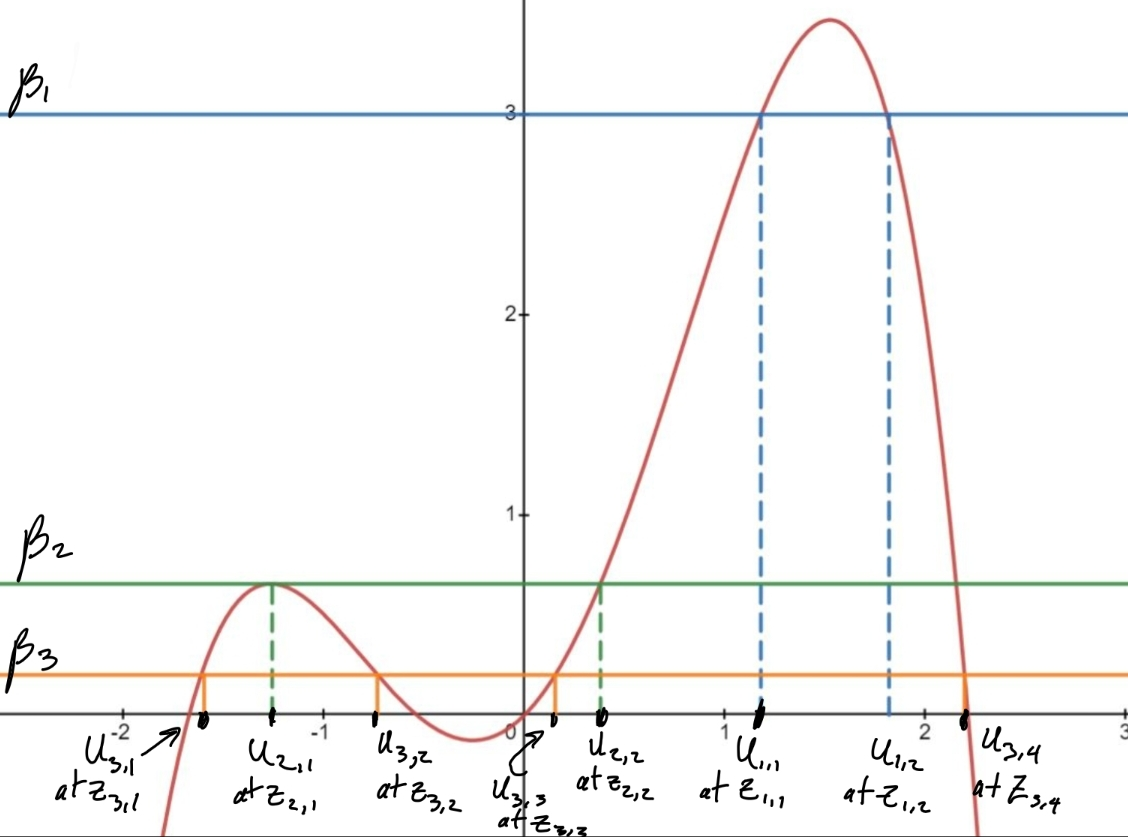
\includegraphics[width=.6\textwidth]{plots/4b-1.jpg}
        \end{center}
        Observe that various $\beta$ values have been plotted that show different maximum potential energy. 
        
        \noindent
        Let's begin by looking at the $\beta_1$ case. In this case there two real valued solutions classes, an elevation solitary wave with $U \in (-\infty, U_{1,1}]$ (seen below to the left) and another elevation solitary wave with $U \in [U_{1,2}, \infty)$ (seen to the right). In both cases it takes a finite amount of time to reach $U_{1,1}$ and $U_{1,2}$.
        \begin{center}
            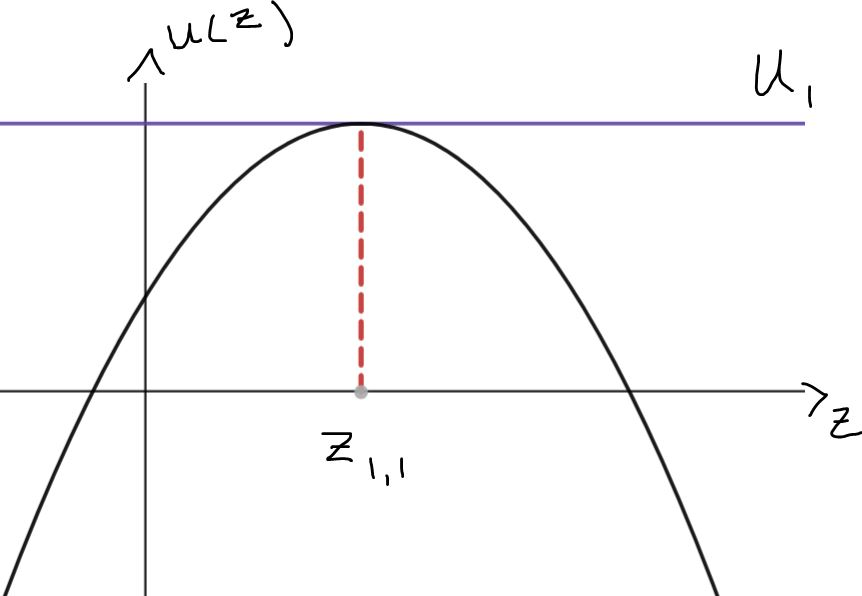
\includegraphics[width=.4\textwidth]{plots/4b-2.JPG}
            \qquad
            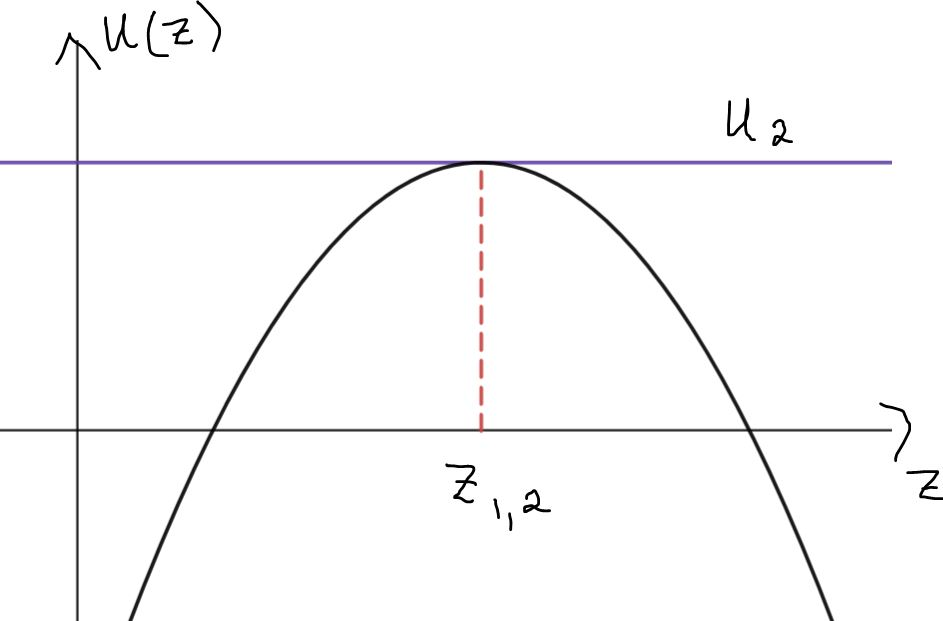
\includegraphics[width=.4\textwidth]{plots/4b-3.JPG}
        \end{center}

        \noindent
        Next let's look at the $\beta_2$ case. There are three real valued solution classes. A solitary solution with $U \in (-\infty,U_{2,1})$ (left), an elevation solitary wave with $U \in (U_{2,1},U_{2,2}]$ (right), and an elevation solitary wave with $U \in [U_{2,3}, \infty)$ (below). In these cases, it takes an infinite amount of time to reach $U_{2,1}$ since it is at a horizontal asymptote while $U_{2,2}$ and $U_{2,3}$ take a finite amount of time to reach.

        \begin{center}
            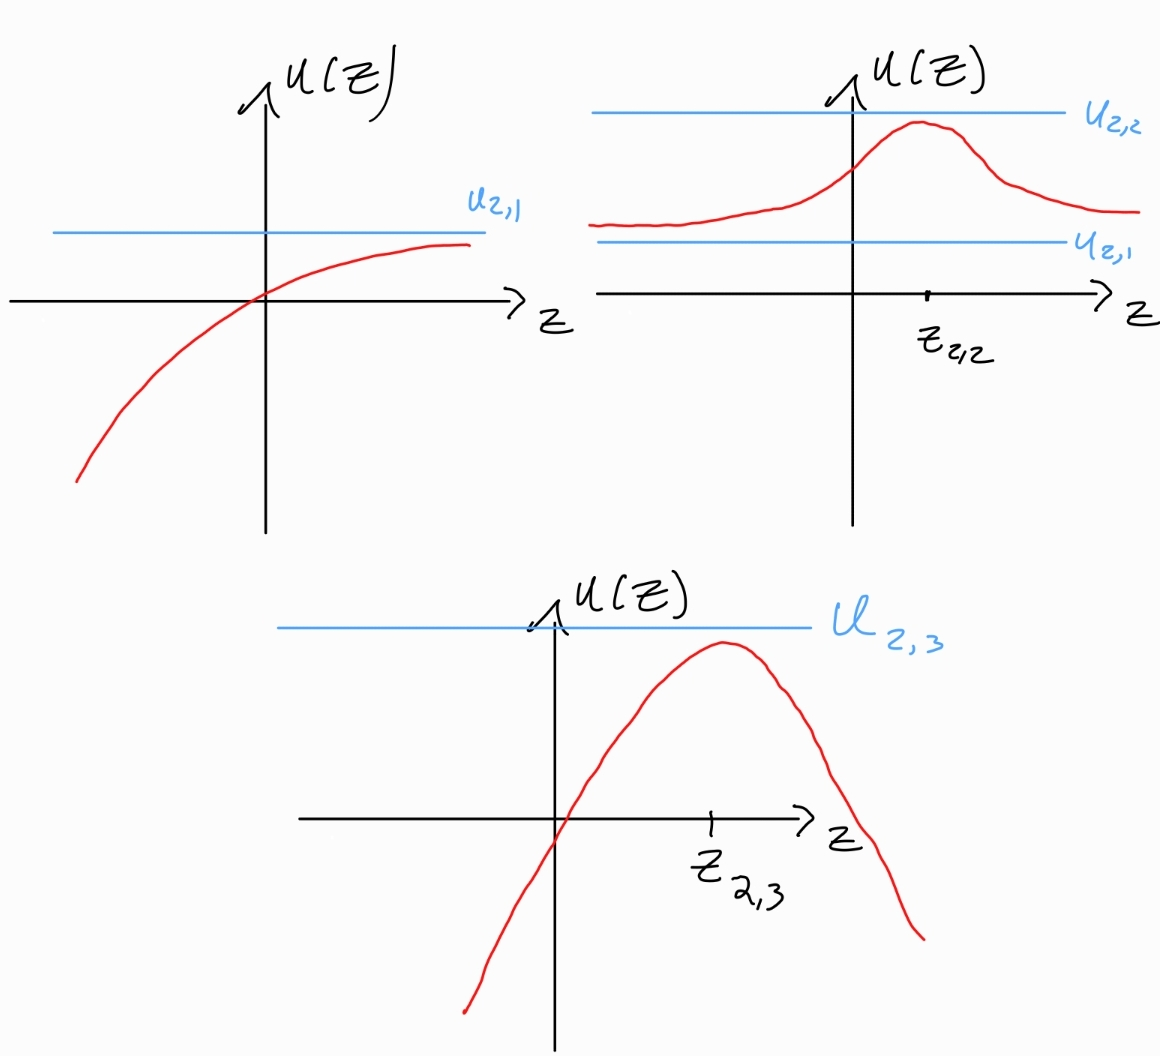
\includegraphics[width=.6\textwidth]{plots/4b-set1.jpg}
        \end{center}

        \noindent
        Next let's look at the $\beta_3$ case. There are three real valued solution classes. One is a solitary elevation wave with $U \in (-\infty, U_{3,1}]$ (left), one is a periodic wave with $U \in [U_{3,2},U_{3,3}]$ (right), and one is a solitary wave with $U \in [U_{3,4},\infty]$ (below). Note that it takes a finite amount of time to each all points $U_{3,1}, \cdots, U_{3,4}$.

        \begin{center}
            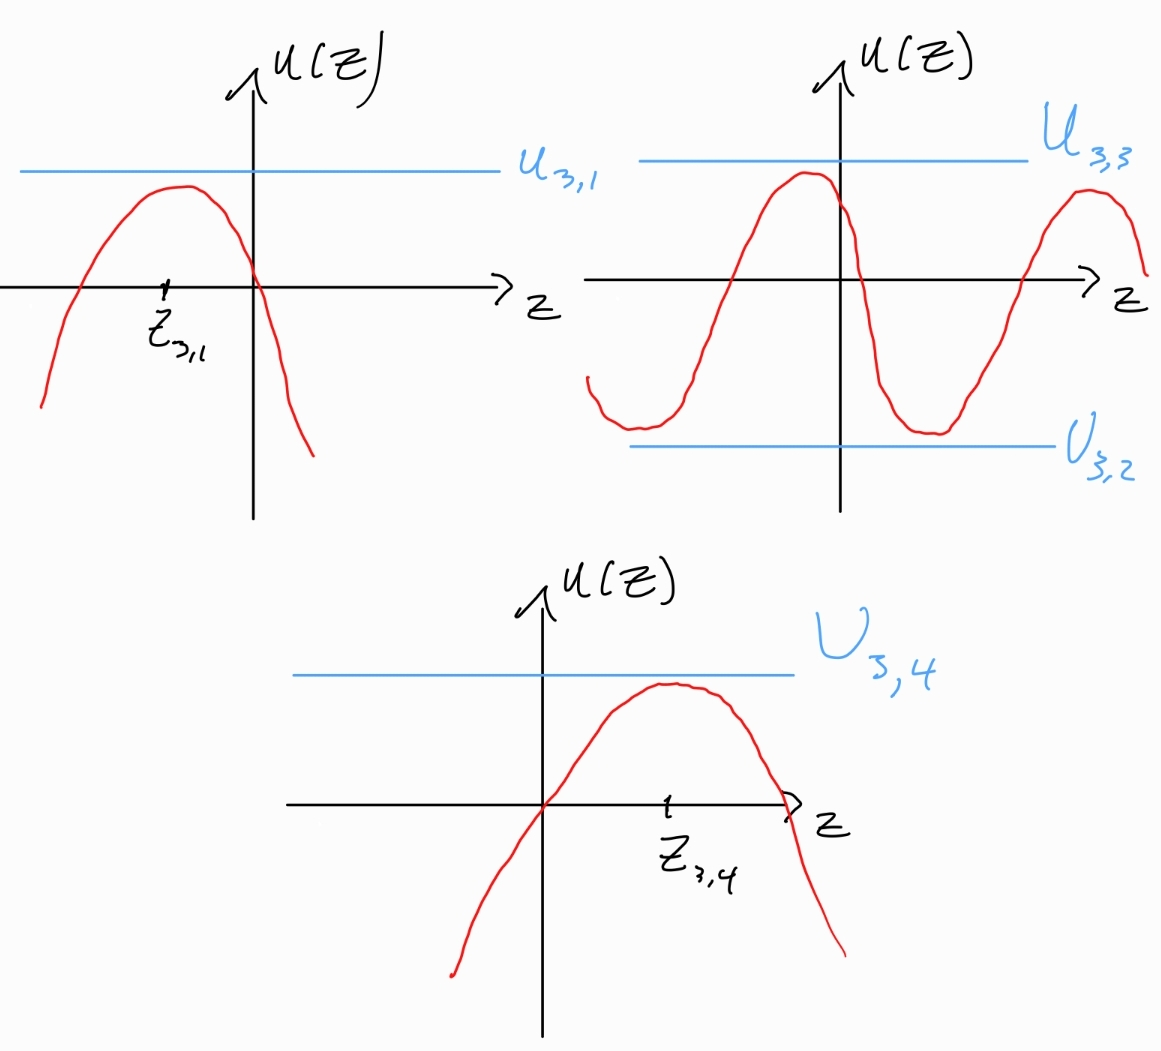
\includegraphics[width=.6\textwidth]{plots/4b-set2.jpg}
        \end{center}

        \noindent
        Finally let's consider the case when $\alpha = 0$. This results in a symmetric solution since both local maximum are at equal heights as seen in the following graph.
        \begin{center}
            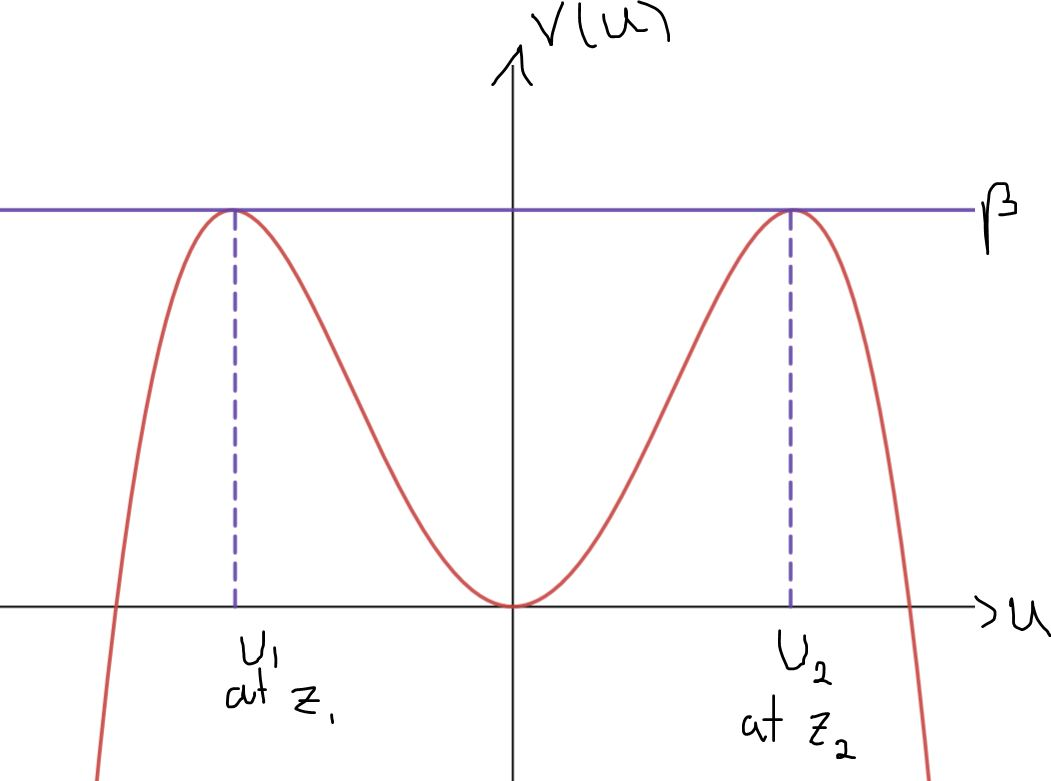
\includegraphics[width=.6\textwidth]{plots/4b-sym.jpg}
        \end{center}
        In this $\beta$ case there are three solution classes. One is a solitary wave with $U \in (-\infty, u_1)$ (left), one is a shock with $U \in (U_1,U_2)$ (right), and one is a solitary wave with $U \in (U_2, \infty)$ (below). Here it takes an infinite amount of time to reach $U_1$ and $U_2$.

        \begin{center}
            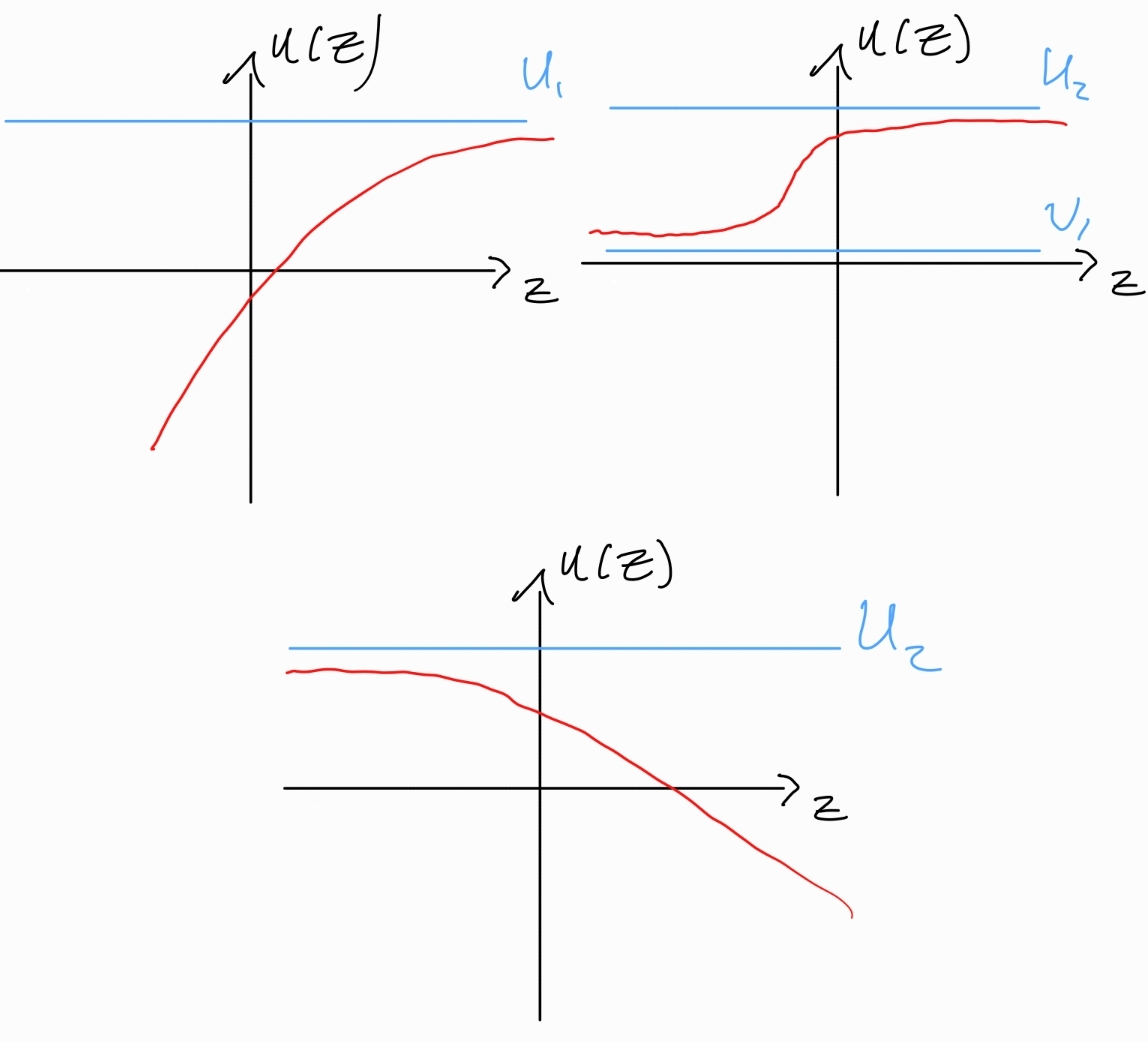
\includegraphics[width=.6\textwidth]{plots/4b-set3.jpg}
        \end{center}

        \noindent
        Next let's consider phase plane analyses. Recall that we found
        \[ 
            -4vU = -2U^3 + U'' + \alpha \implies U'' = -4vU + + 2U^3 - \alpha.
        \]
        If we let $u_1 = U$ and $u_2 = U'$ then we get the system
        \begin{align*}
            u_1' &= u_2\\
            u_2 &= -4vu_1 + 2u_1^3 - \alpha = -\pp{V(u_1)}{u_1},
        \end{align*}
        where $V(u) = \alpha u + 2vu^2 - \half u^4$. Thus we have a ODE dynamical system and we see that the equilibrium will have solutions of the form of the critical points of the potential equation
        \[ 
            \pp{v}{u} = -2U^3 + 4vU + \alpha = 0.
        \]
        Since this is a cubic equation with real coefficients we will always have at least one real root. To find the cases, recall that the discriminant is given by,
        \begin{align*}
            \Delta &= -4ac^3 - 27a^2d^2 = 512v^3 - 108\alpha^2.
        \end{align*}
        So when $\Delta > 0$ there will be two potential hills and one well (3 equilibrium points), let's call this case 3. When $\Delta \to 0$, one potential hill goes away, leaving a horizontal tangent (2 equilibrium points), let's call this case 2. And When $\Delta < 0$ there will be one potential hill (1 equilibrium point), let's call this case 1. Each of the cases can be seen in the following graphs where $v=1$ and $\alpha =1$.   
        \begin{center}
            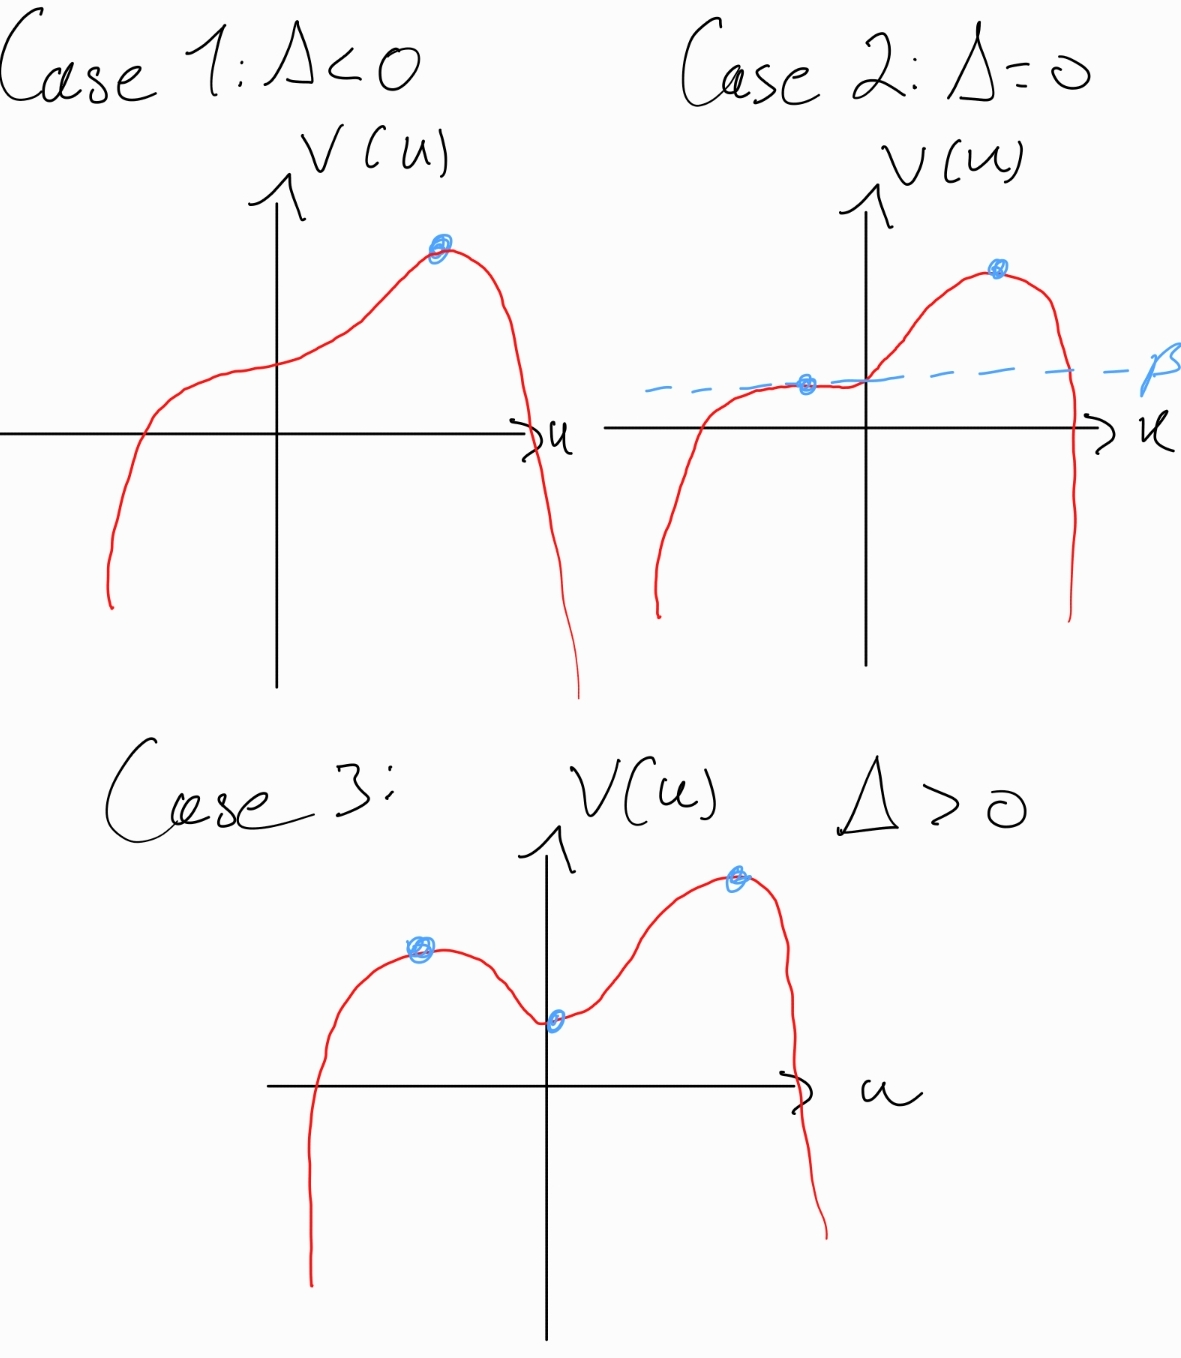
\includegraphics[width=.6\textwidth]{plots/4b-situations.jpg}
        \end{center}

        \noindent 
        Let's consider case 1: $\Delta < 0$. In this case we expect to find that all solutions move away from the equilibrium position since it is a hill. Letting $\alpha = 1$ and $v=1$ we can see that the phase potrait looks like the following phase plane.

        \begin{center}
            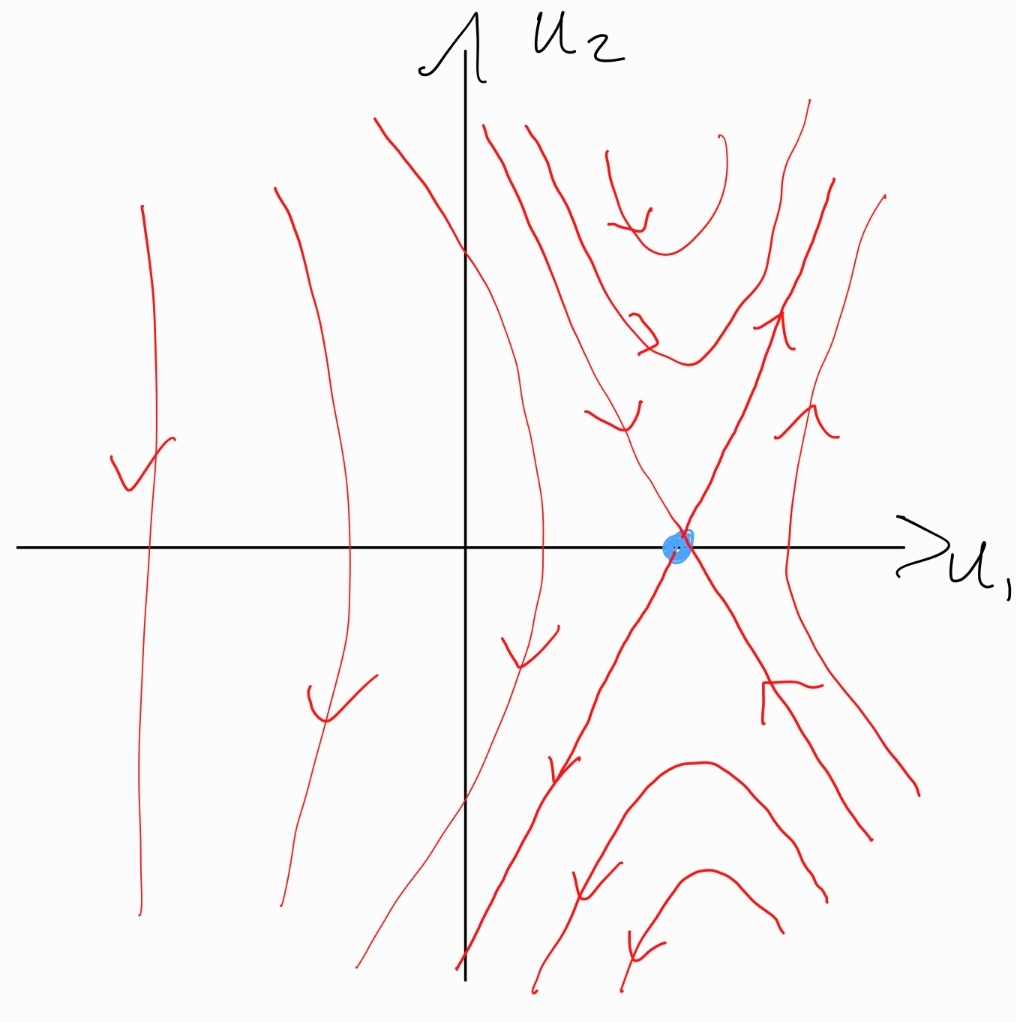
\includegraphics[width=.6\textwidth]{plots/4b-phase1.jpg}
        \end{center}        

        \noindent 
        Let's consider case 2: $\Delta = 0$. For $\Delta = 0$, let $\alpha = 1$ and then $v = \frac{3}{4(2)^{\frac{3}{2}}}$. We expect to have similar behavior as before around the maximum critical points but we also have a horizontal tangent critical point which degenerates. Thus we come up with the following phase plane.

        \begin{center}
            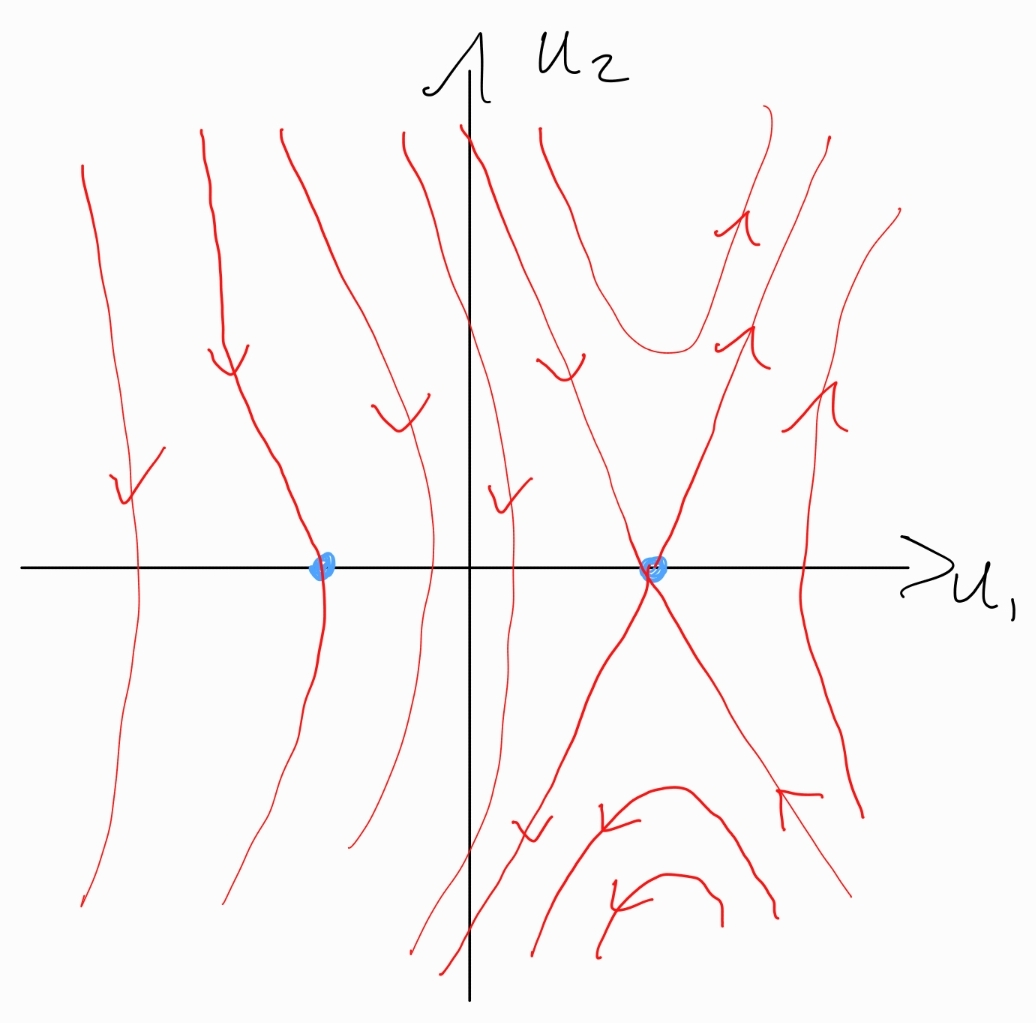
\includegraphics[width=.6\textwidth]{plots/4b-phase2.jpg}
        \end{center}

        \noindent 
        Let's consider case 3: $\Delta > 0$. In this case, there will be two different scenarios. One where the local maximum critical points are not equal (i.e. $\alpha \neq 0$) and the other where the local maximum are at equal heights (i.e. $\alpha = 0$). Let's first consider when maximum are unequal. Let's let $v=1$ and $\alpha = 1$. We expect solutions on the outer side of the hills to run to infinity while there is a different behavior around the well between the hills. We noted before that the well will have periodic solutions and thus we expect a center type critical point. Note that we can observe a homoclinic orbit at the left hill. 

        \begin{center}
            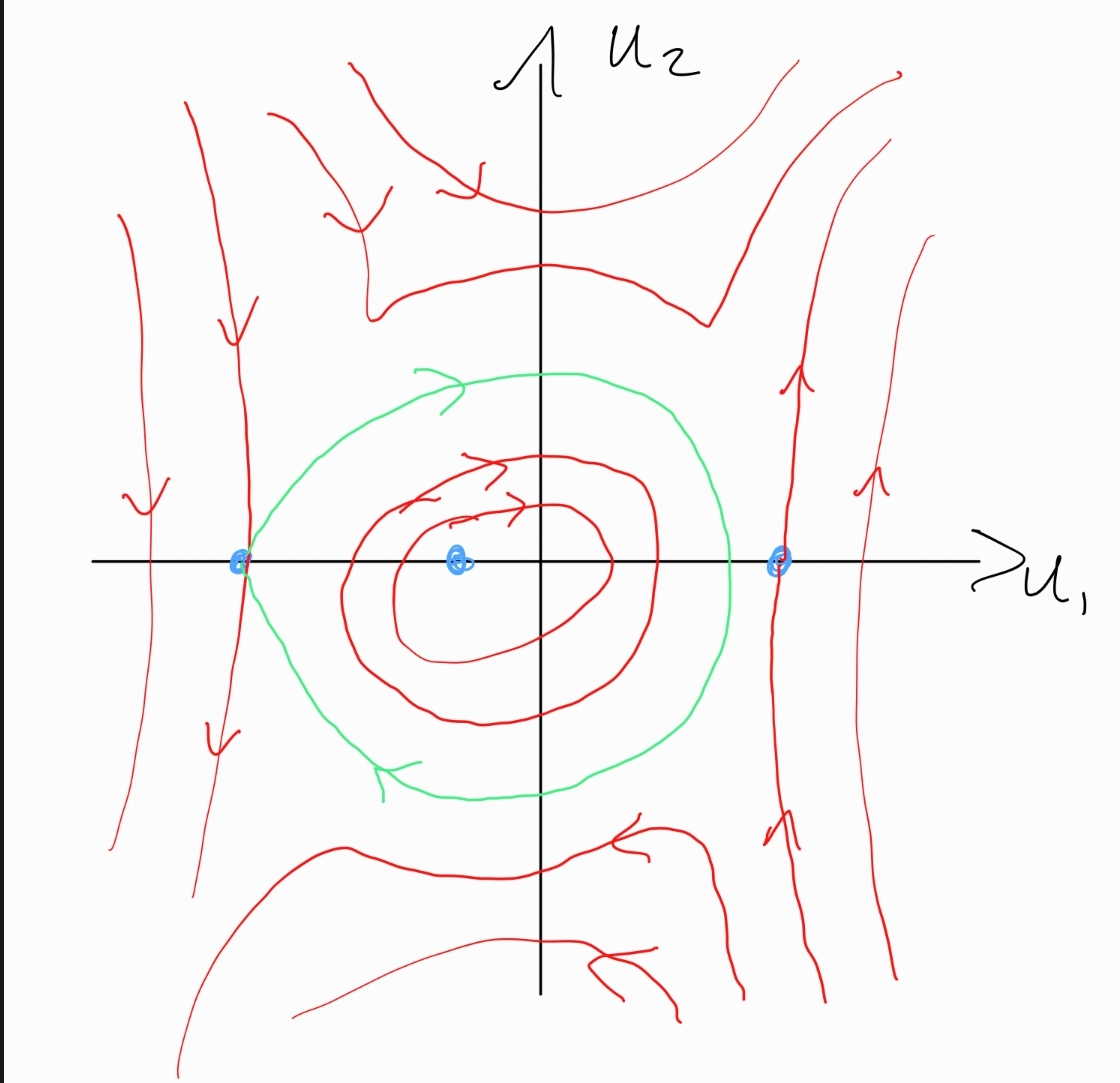
\includegraphics[width=.6\textwidth]{plots/4b-phase3.jpg}
        \end{center}

        Now consider the scenario where $\alpha =0$ and let $v=1$. In this case we have similar behavior as before except a heteroclinic orbit arises between the two hills. This correlates with the previous observation we made of when $\alpha = 0$ a shock wave arises rather than a periodic wave.  
        
        \begin{center}
            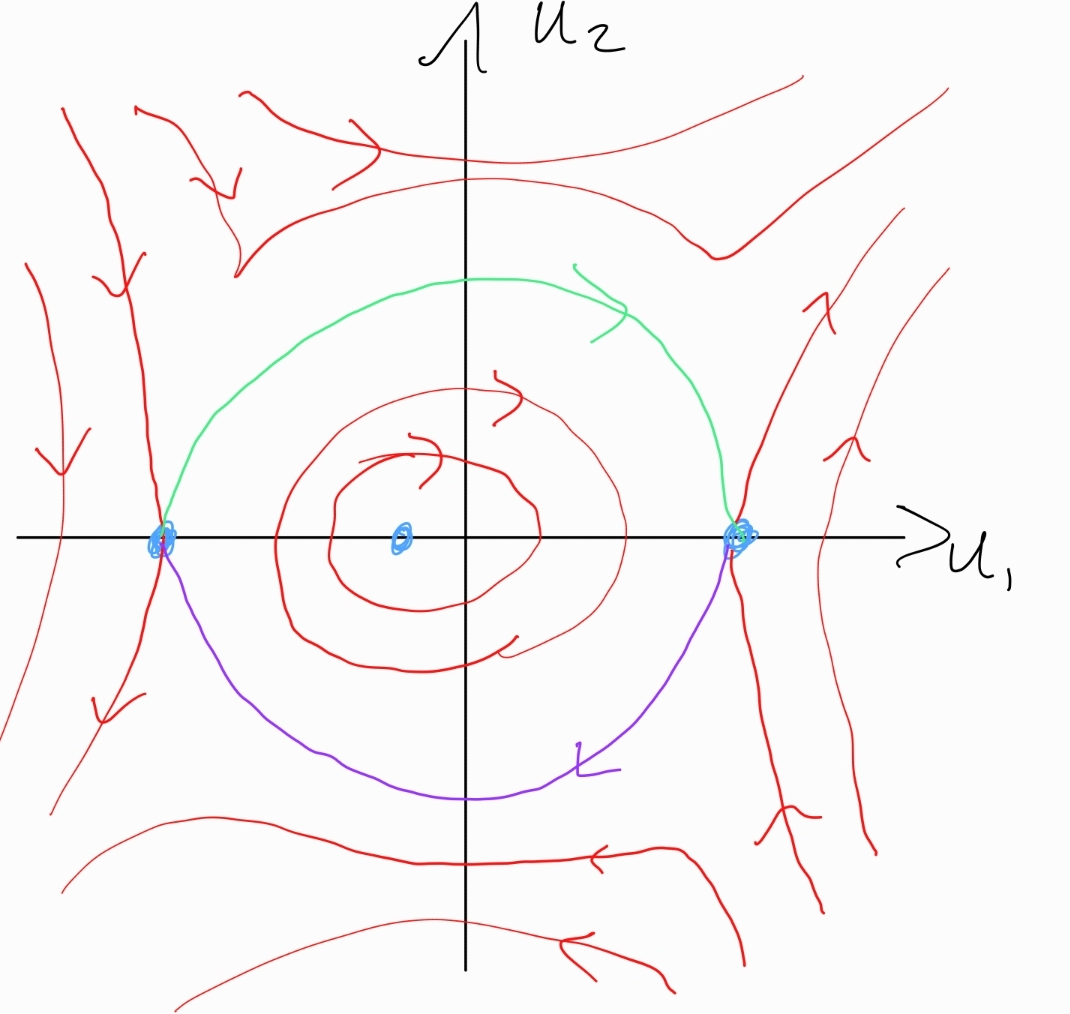
\includegraphics[width=.6\textwidth]{plots/4b-phase4.jpg}
        \end{center}

        \item[{\bf b.}]
        Now we want to obtain the explicit functional form of the solution. Recall the potential energy equation,
        \[ 
            \frac{1}{2}U'^2 + V(u) = \beta,
        \]
        which we can solve to get
        \[
            u' = \pm \sqrt{2(\beta - V(u))}.
        \]
        Now we can separate variables to get an implicit solution 
        \[
            \pm\int_{u_0}^u \frac{du}{\sqrt{2(\beta - V(u))}} = \pm \int_0^zdz = \pm z.
        \]
        Thus we have obtained the implicit solution to be,
        \[
            \pm z = \int_{u_0}^u \frac{du}{\sqrt{2(\beta - V(u))}}.
        \]
        Now we will not consider the homoclinical case but rather focus on the heteroclinical case. The heteroclinical case only occurs when $V$ is symmetric and the local maximums are equal, i.e. when $\alpha = 0$. Thus the potential energy function reduces to
        \[
        V(u) = 2vu^2 - \frac{1}{2}u^4. 
        \]
        To find the maximum height, consider that
        \begin{align*}
            \pp{v}{u} = 4vU - 2u^3 = 0 \implies u^2 = 2v \implies u = \pm \sqrt{2v}.
        \end{align*}
        By definition of the heteroclinic orbit, we know that $u \to \pm \sqrt{2v}$ as $x \to \pm \infty$. We also note that all derivatives of $u$ are to zero as $x \to \infty$. Knowing these facts we can now solve for the value of $\beta$ by solving the equation
        \begin{align*}
            -2vU^2 &= \frac{-U^4}{2} + \frac{U'^2}{2} + \alpha U - \beta\\
            \implies -2v(2v) &= \frac{-4v^2}{2} - \beta\\
            \implies \beta &= 2v^2.
        \end{align*}
        We are now able to further evaluate our implicit integral using that $\alpha = 0$ and $\beta = 2v^2$
        \begin{align*}
            \pm z &= \int_{u_0}^u \frac{du}{\sqrt{2(\beta - V(u))}}\\
            \pm z &= \int_{u_0}^u \frac{du}{\sqrt{2(2v^2 + \frac{1}{2}u^4 - 2vU^2)}}\\
            \pm z &= \int_{u_0}^u \frac{du}{\sqrt{4v^2 + U^4 - 4vU2}}.\\
        \end{align*}
        Using Mathematica to compute this integral we get
        \begin{align*}
            \pm z &= - \frac{1}{\sqrt{2v}}\tanh^{-1}\paren{\frac{u}{\sqrt{2v}}} |_{u_0}^u\\
            &= -\frac{1}{2v}\paren{\tanh^{-1}\paren{\frac{u}{\sqrt{2v}}}-\tanh^{-1}\paren{\frac{u_0}{\sqrt{2v}}}}.
        \end{align*}
        We can now solve for $u$ as follows
        \begin{align*}
            -\frac{1}{2v}\paren{\tanh^{-1}\paren{\frac{u}{\sqrt{2v}}}} &= \pm z -  \frac{1}{2v}\paren{\tanh^{-1}\paren{\frac{u_0}{\sqrt{2v}}}}\\
            \tanh^{-1}\paren{\frac{u}{\sqrt{2v}}} &= \mp \sqrt{2v} z -  \tanh^{-1}\paren{\frac{u_0}{\sqrt{2v}}}\\
            \frac{u}{\sqrt{2v}} &= \tanh\paren{\mp \sqrt{2v} z -  \tanh^{-1}\paren{\frac{u_0}{\sqrt{2v}}}}\\
            u &= \sqrt{2v}\tanh\paren{\mp \sqrt{2v} z -  \tanh^{-1}\paren{\frac{u_0}{\sqrt{2v}}}},\\
        \end{align*}
        and if we let $\tanh^{-1}\paren{\frac{u_0}{\sqrt{2v}}} = -\sqrt{2v}x_0$ we get that
        \[
            u(x,t) = \sqrt{2v}\tanh(\mp\sqrt{2v}z - \sqrt{2v}x_0) = \sqrt{2v}\tanh(\sqrt{2v}(\mp z - x_0)). 
        \]
        Recalling that we let $u(x,t) = U(x-vt)$, we have found an explicit solution for the heteroclinic orbit to be
        \[
            u(x,t) = \sqrt{2v}\tanh(\sqrt{2v}(x - x_0 \mp v t)).
        \]
    \end{enumerate}
\end{solution}

\end{document}